\chapter{Definición de Arquitectura}

En este capítulo, después de haber definido los requerimientos (Tabla \ref{tab:requerimientos-eps}), nos adentramos en la fase de diseño del sistema. La creación de una representación clara y significativa del sistema es de suma importancia en este proceso. Para lograrlo, debemos considerar dos enfoques fundamentales ampliamente utilizados en el campo de la ingeniería: el enfoque \emph{bottom-up} (de abajo hacia arriba) y el enfoque \emph{top-down} (de arriba hacia abajo) \cite{ford2008design}.

\hspace{1.27cm}En el enfoque \emph{bottom-up}, comenzamos con componentes básicos que se ensamblan gradualmente para formar el sistema completo. Podemos pensar en esto como la construcción de un automóvil a partir de neumáticos, motor, chasis y otros elementos fundamentales. Este enfoque nos insta a prestar atención a los detalles mientras construimos el sistema, manteniendo la simplicidad sin caer en niveles excesivos de profundidad.

\hspace{1.27cm}Por otro lado, el enfoque \emph{top-down} nos invita a partir de una visión general del sistema final. Dividimos este sistema en partes y subsistemas que trabajan en conjunto para alcanzar el objetivo general. Este método nos permite mantener una perspectiva amplia y clara, definiendo primero los componentes principales antes de adentrarnos en los detalles más finos.

\hspace{1.27cm}Al aplicar estos enfoques, debemos recordar que nuestro objetivo es definir un nivel base de funcionalidad. No debemos caer en la trampa de una profundización excesiva que podría llevar a complicaciones innecesarias. 

\hspace{1.27cm}En nuestro proceso de diseño, además, evaluamos modelos previos y valoramos factores de innovación y escalabilidad. Esta estrategia nos habilita para edificar sobre conocimientos previos y estar preparados para futuras mejoras en el sistema. Para los propósitos de esta tesis, hemos optado por implementar el enfoque \emph{Top-Down} utilizando diagramas y tablas que muestran las entradas y salidas par cada bloque funcional según los niveles de profundidad.
\newpage


%Decomposición funcional: Nivel 0

\section{Nivel 0}

\begin{figure}[h!]
\centering
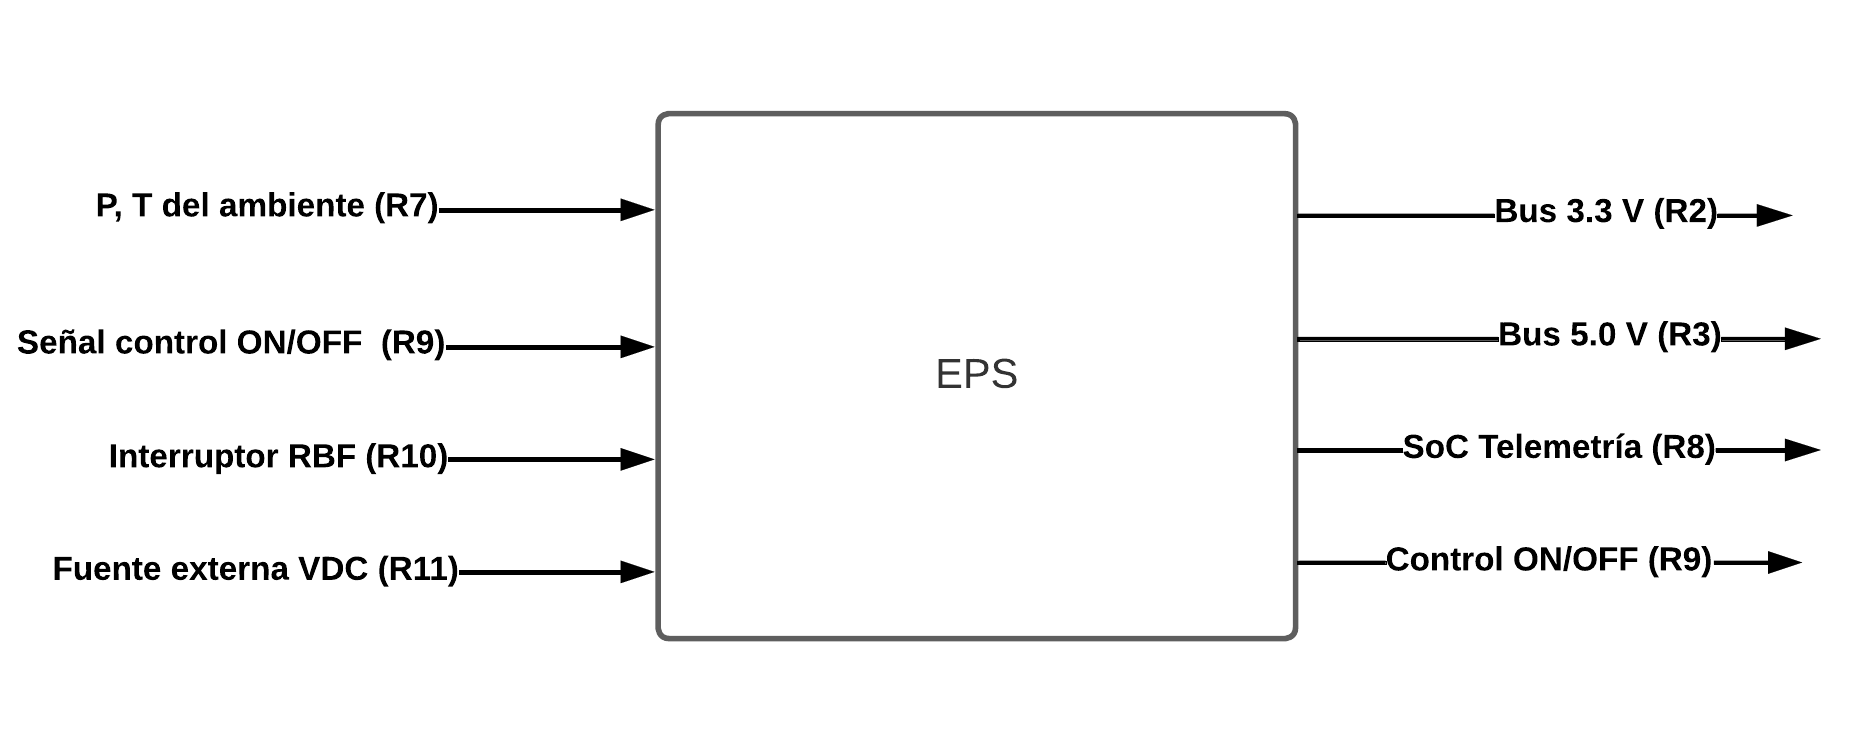
\includegraphics[width=\textwidth]{Pictures/Level0.png}
\caption{Diagrama funcional Nivel 0.}\label{fig:Level0}
\index{figures}
\end{figure}

\begin{table}[h]
    \centering
    \caption{Detalles de Nivel 0}
    \label{tab:nivel0}
    \begin{tabular}{ll}
    \toprule
        Módulo  & Electrical Power System (EPS) \\ 
    \midrule
        Entradas & 
        \begin{minipage}[t]{0.75\linewidth}
        - Presión atmosférica y temperatura ambiente. \\
        - Señales de navegación para control ON/OFF de carga útil. \\
        - Señal de interruptor RBF (Remove before flight).\\
        - Fuente externa VDC para el cargador de baterías.
        \end{minipage} \\
    \midrule
        Salidas & 
        \begin{minipage}[t]{0.75\linewidth}
        - Bus 3.3 V $\pm$ 1\%, 1.5A (factor de seguridad 1.25) \\
        - Bus 5.0 V $\pm$ 1\%, 0.6A factor de seguridad 1.25)\\
        - Estado de carga de baterías (SoC) \\
        - Control ON/OFF para carga útil, 5V $\pm$ 1\%
        \end{minipage} \\
    \midrule
        Funcionamiento & 
        \begin{minipage}[t]{0.75\linewidth}
El sistema se activa mediante un interruptor RBF y se alimenta con baterías de iones de litio 18650 recargadas por una fuente externa de VDC. Recopila datos de voltaje, corriente, presión atmosférica y temperatura ambiental, y proporciona dos buses de alimentación a 3.3 V y 5.0 V. Además, transmite el estado de carga de las baterías (SoC) al subsistema de telemetría y suministra energía a la carga útil bajo el control del subsistema de navegación.

        \end{minipage} \\
    \bottomrule
    \end{tabular}
\end{table}

\newpage

%Decomposición funcional: Nivel 1
%-**************************************

\section{Nivel 1}

\begin{figure}[h!]
\centering
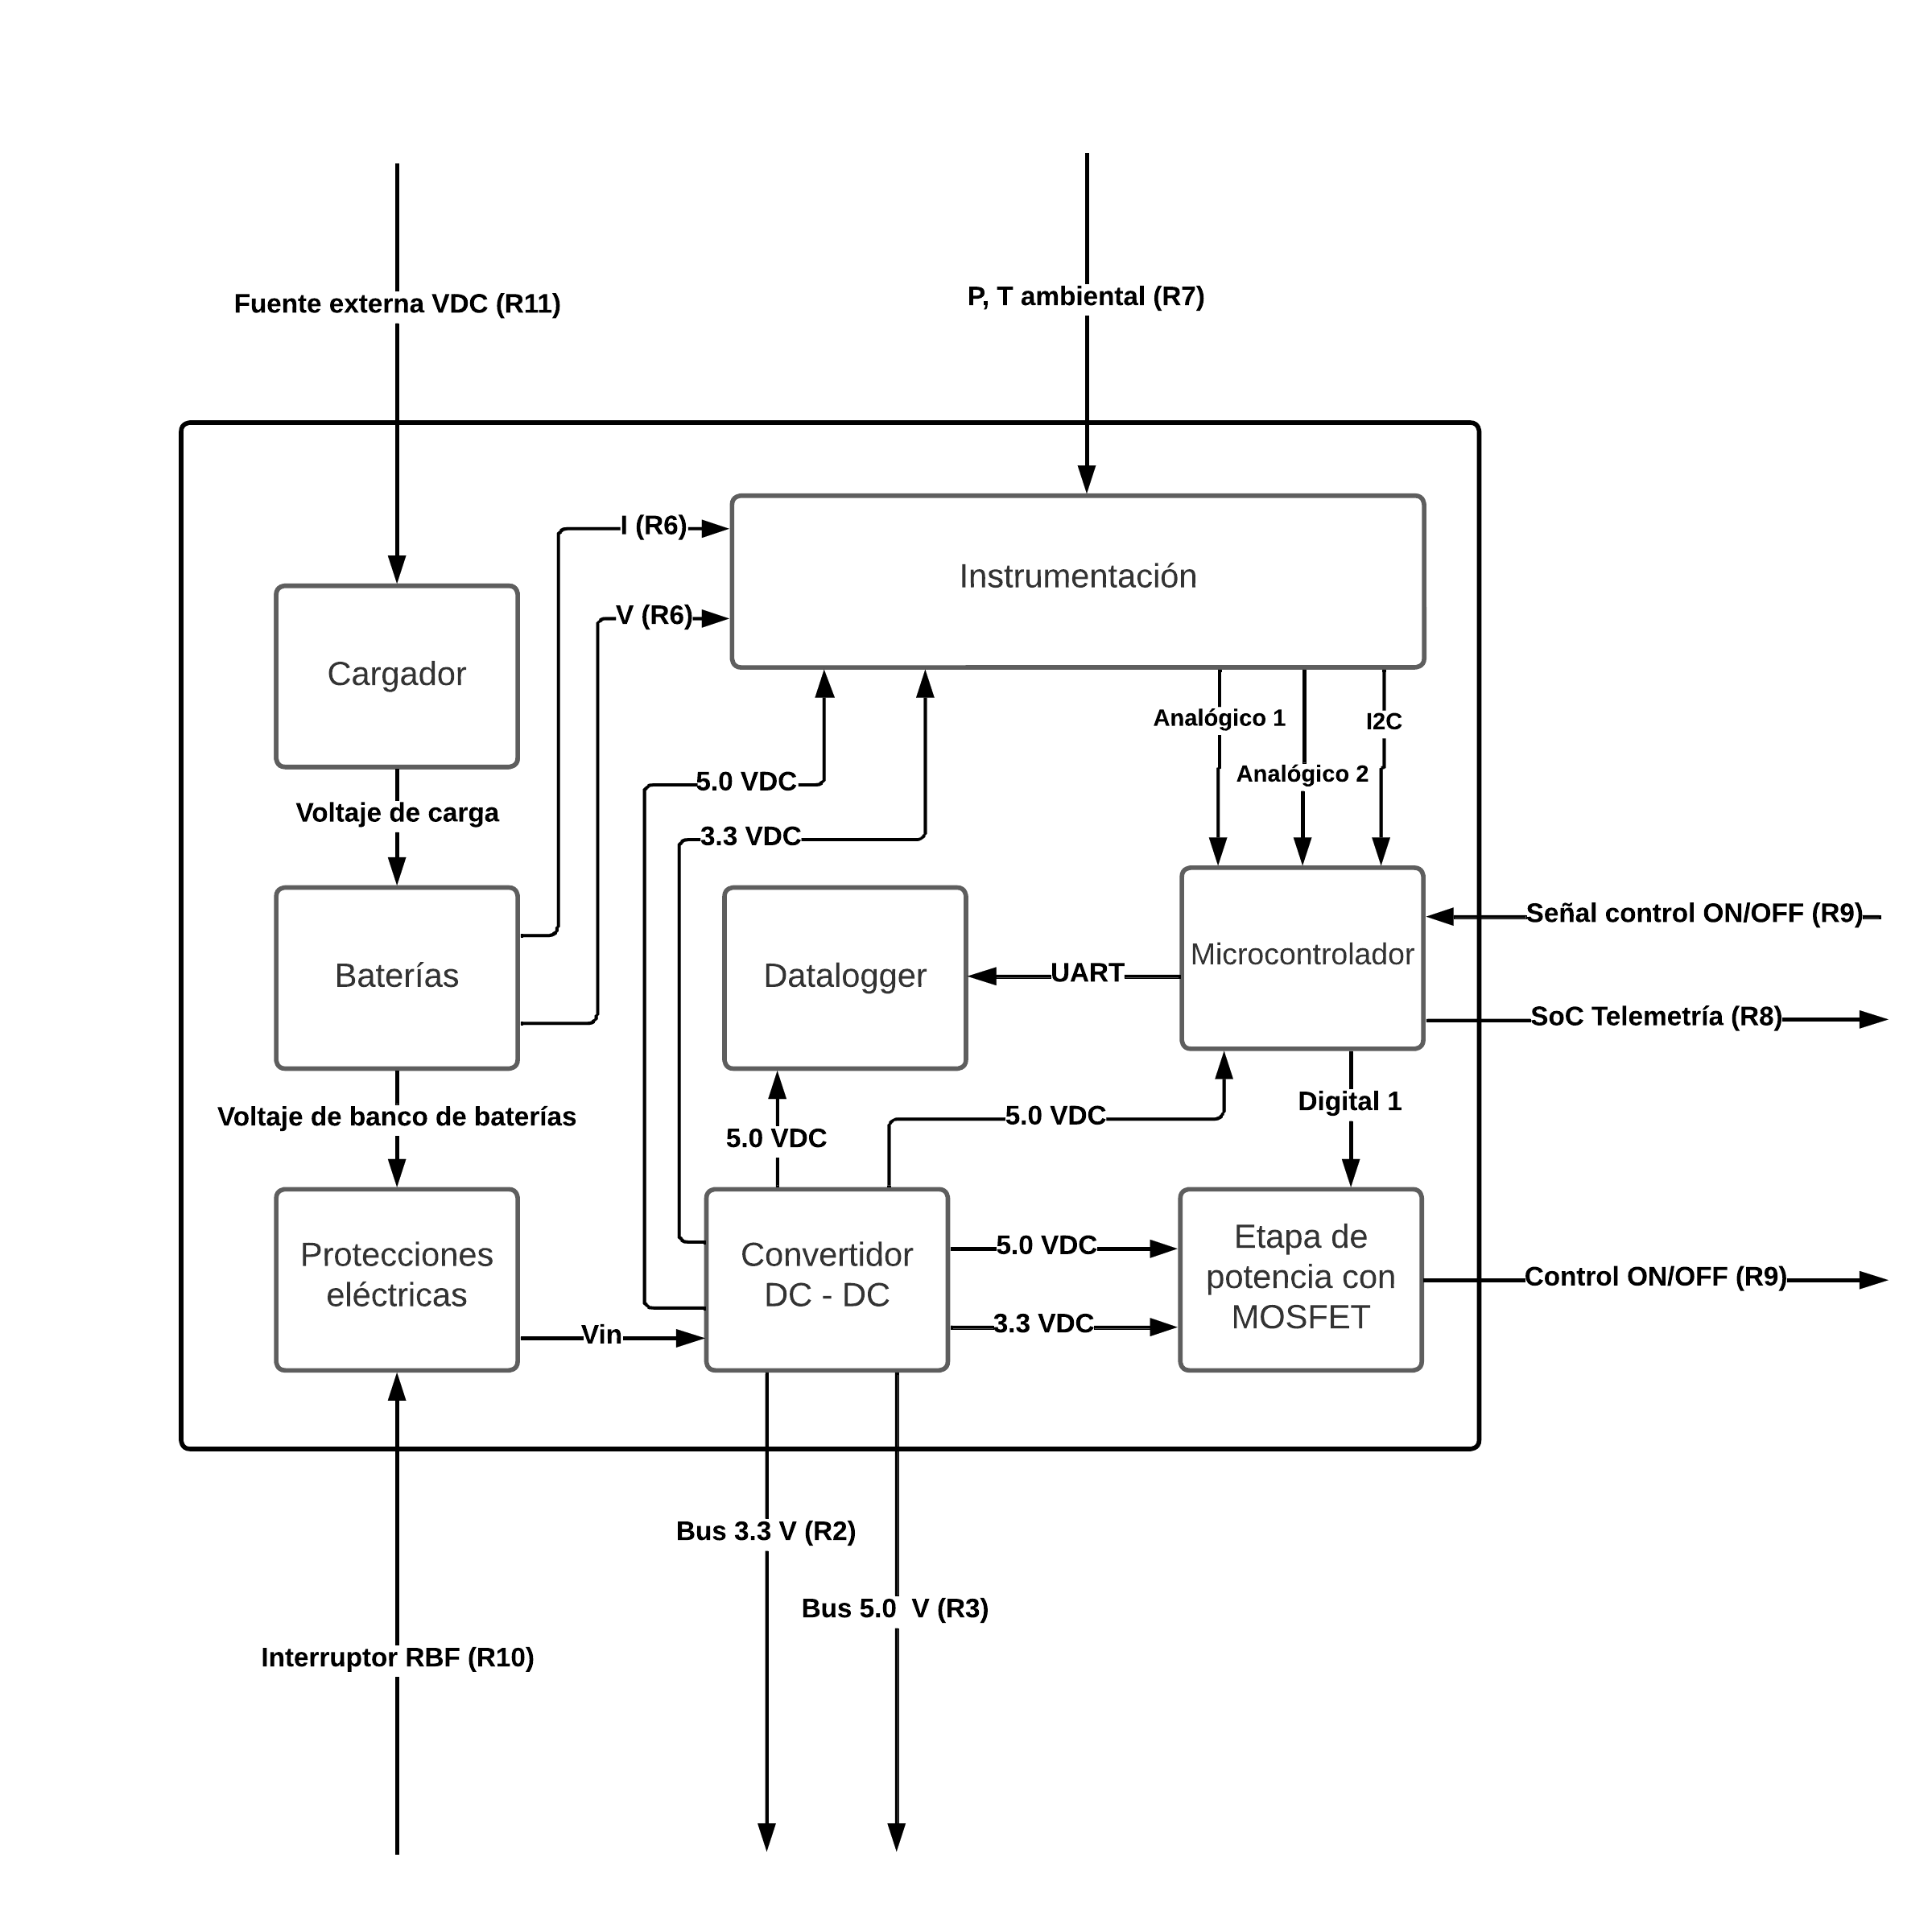
\includegraphics[width=0.8\textwidth]{Pictures/Level1.png}
\caption{Diagrama funcional Nivel 1.}\label{fig:Level1}
\index{figures}
\end{figure}

\begin{table}[h!]
    \centering
    \caption{Detalles de Nivel 1, cargador.}
    \label{tab:nivel1_cargador}
    \begin{tabular}{ll}
    \toprule
        Módulo  & Cargador\\ 
    \midrule
        Entradas & 
        \begin{minipage}[t]{0.75\linewidth}
 - Fuente externa VDC 5.0 V $\pm$ 1\% 
        \end{minipage} \\
    \midrule
        Salidas & 
        \begin{minipage}[t]{0.75\linewidth}
        - Voltaje de carga (4.2 v $\pm$ 1\%) para baterías Li-ion 18650.
        \end{minipage} \\
    \midrule
        Funcionamiento & 
        \begin{minipage}[t]{0.75\linewidth}
El cargador recibe energía de una fuente externa de tensión constante (\textit{VDC}). Su función principal es proporcionar una salida de $4.2 \, \text{V} \pm 1\%$ para cargar baterías de ion de litio 18650.

        \end{minipage} \\
    \bottomrule
    \end{tabular}
\end{table}
\newpage

%-**************************************
% BATERÍAS 
\begin{table}[!ht]
    \centering
    \caption{Detalles de Nivel 1, baterías.}
    \label{tab:nivel1_baterias}
    \begin{tabular}{ll}
    \toprule
        Módulo  & Baterías\\ 
    \midrule
        Entradas & 
        \begin{minipage}[t]{0.75\linewidth}
 - Voltaje de carga a $4.2 \, \text{V} \pm 1\%$ 
        \end{minipage} \\
    \midrule
        Salidas & 
        \begin{minipage}[t]{0.75\linewidth}
- El voltaje de salida del banco de baterías se determina mediante una configuración serie-paralelo de pilas con un voltaje nominal de 3.6 V.

        \end{minipage} \\
    \midrule
        Funcionamiento & 
        \begin{minipage}[t]{0.75\linewidth}
El banco de baterías tiene la función de entregar la potencia eléctrica requerida por el EPS.

        \end{minipage} \\
    \bottomrule
    \end{tabular}
\end{table}


%-**************************************

% PROTECCIONES ELÉCTRICAS

\begin{table}[h!]
    \centering
    \caption{Detalles de Nivel 1, protecciones eléctricas.}
    \label{tab:nivel1_protecciones}
    \begin{tabular}{ll}
    \toprule
        Módulo  & Protecciones Eléctricas\\ 
    \midrule
        Entradas & 
        \begin{minipage}[t]{0.75\linewidth}
 - Voltaje del banco de baterías.\\ - Señal de activación de interruptor RBF.
 
        \end{minipage} \\
    \midrule
        Salidas & 
        \begin{minipage}[t]{0.75\linewidth}
- Voltaje de entrada para etapa de regulación de voltaje.

        \end{minipage} \\
    \midrule
        Funcionamiento & 
        \begin{minipage}[t]{0.75\linewidth}
Consta de una protección tipo "Remove before Flight" y un interruptor de 4 polos para la desconexión de las pilas 18650.

        \end{minipage} \\
    \bottomrule
    \end{tabular}
\end{table}
%-**************************************

% REGULACIÓN DE VOLTAJE
\begin{table}[h!]
    \centering
    \caption{Detalles de Nivel 1, Convertidor DC-DC.}
    \label{tab:nivel1_protecciones}
    \begin{tabular}{ll}
    \toprule
        Módulo  & Convertidor DC-DC\\ 
    \midrule
        Entradas & 
        \begin{minipage}[t]{0.75\linewidth}
 - Voltaje del banco de baterías.
 
        \end{minipage} \\
    \midrule
        Salidas & 
        \begin{minipage}[t]{0.75\linewidth}
- Bus 3.3 V $\pm$ 1\%, 1.5A (factor de seguridad 1.25) \\
        - Bus 5.0 V $\pm$ 1\%, 0.6A factor de seguridad 1.25)\\

        \end{minipage} \\
    \midrule
        Funcionamiento & 
        \begin{minipage}[t]{0.75\linewidth}
La etapa de convertidores DC-DC transforma el voltaje de las pilas Li-ion 18650 del banco de baterías en dos buses de salida: uno de $5.0 \, \text{V} \pm 1\%$ que suministra al menos 983 mA y otro de $3.3 \, \text{V} \pm 1\%$ con una capacidad mínima de 402.30 mA. Estos buses alimentan los subsistemas electrónicos y las cargas del sistema.


        \end{minipage} \\
    \bottomrule
    \end{tabular}
\end{table}

%-**************************************

% ETAPA DE POTENCIA MOSFET

\begin{table}[h!]
    \centering
    \caption{Detalles de Nivel 1, etapa de potencia con MOSFET.}
    \label{tab:nivel1_MOSFET}
    \begin{tabular}{ll}
    \toprule
        Módulo  & Etapa de potencia con MOSFET\\ 
    \midrule
        Entradas & 
        \begin{minipage}[t]{0.75\linewidth}
 - Alimentación $5.0 \, \text{V} \pm 1\%$\\
 - Alimentación $3.3 \, \text{V} \pm 1\%$\\
 - Señal digital de activación de microcontrolador (Digital 1)
 
        \end{minipage} \\
    \midrule
        Salidas & 
        \begin{minipage}[t]{0.75\linewidth}
    - Control de activación ON/OFF a tensión $5.0 \, \text{V} \pm 1\%$

        \end{minipage} \\
    \midrule
        Funcionamiento & 
        \begin{minipage}[t]{0.75\linewidth}
Activa o desactiva la fuente de alimentación de la caerga útil. 

        \end{minipage} \\
    \bottomrule
    \end{tabular}
\end{table}

\vspace{4 cm}
%****************************************
% Microcontrolador

\begin{table}[h!]
    \centering
    \caption{Detalles de Nivel 1, microcontrolador.}
    \label{tab:nivel1_Microcontrolador}
    \begin{tabular}{ll}
    \toprule
        Módulo  & Microcontrolador\\ 
    \midrule
        Entradas & 
        \begin{minipage}[t]{0.75\linewidth}
 - Alimentación $5.0 \, \text{V} \pm 1\%$\\
 - Señal de activación para control ON/OFF proveniente de subsistema de Navegación vía I2C.\\
- Señal analógica 1 de etapa de instrumentación.\\
- Señal analógica 2 de etapa de instrumentación.\\
- Comunicación I2C de etapa de instrumentación.\\
 
        \end{minipage} \\
    \midrule
        Salidas & 
        \begin{minipage}[t]{0.75\linewidth}
    - Comunicación UART con Datalogger.\\
    - Señal digital de activación de microcontrolador (Digital 1)\\
    - Estado de carga (SoC) para subsistema de Telemetría vía I2C.

        \end{minipage} \\
    \midrule
        Funcionamiento & 
        \begin{minipage}[t]{0.75\linewidth}
El microcontrolador se alimenta con una tensión de $5.0 \, \text{V} \pm 1\%$. Recibe lecturas analógicas (1 y 2) de la etapa de instrumentación, así como datos a través de la comunicación I2C. Además, recibe una señal digital del subsistema de Navegación, la cual está asociada a un control ON/OFF para la activación de la carga útil.

En lo que respecta a las salidas, envía datos de registro al Datalogger a través de una conexión UART. Utiliza el pin Digital 1 para activar o desactivar la etapa de potencia que alimenta la carga útil. Finalmente, después de un procesamiento interno, el microcontrolador calcula y transmite vía I2C el estado de carga (SoC) al subsistema de telemetría.


        \end{minipage} \\
    \bottomrule
    \end{tabular}
\end{table}

%***************************************
% Datalogger
% Microcontrolador

\begin{table}[h!]
    \centering
    \caption{Detalles de Nivel 1, Datalogger.}
    \label{tab:nivel1_Datalogger}
    \begin{tabular}{ll}
    \toprule
        Módulo  & Datalogger\\ 
    \midrule
        Entradas & 
        \begin{minipage}[t]{0.75\linewidth}
 - Alimentación $5.0 \, \text{V} \pm 1\%$\\
 - Recepción de datos vía UART, provenientes del Microcontrolador.
 
        \end{minipage} \\
    \midrule
        Salidas & 
        \begin{minipage}[t]{0.75\linewidth}
    - Registro de datos en MicroSD

        \end{minipage} \\
    \midrule
        Funcionamiento & 
        \begin{minipage}[t]{0.75\linewidth}
El datalogger alimentado a  $5.0 \, \text{V} \pm 1\%$ recibe datos vía UART y los registra en una MicroSD.

        \end{minipage} \\
    \bottomrule
    \end{tabular}
\end{table}
% ESPACIADO VERTICAL
\vspace{4 cm}
%***************************************
% INSTRUMENTACIÓN

\begin{table}[h!]
    \centering
    \caption{Detalles de Nivel 1, Instrumentación.}
    \label{tab:nivel1_Instrumentacion}
    \begin{tabular}{ll}
    \toprule
        Módulo  & Instrumentación\\ 
    \midrule
        Entradas & 
        \begin{minipage}[t]{0.75\linewidth}
  - Alimentación $5.0 \, \text{V} \pm 1\%$\\
   - Alimentación $3.3 \, \text{V} \pm 1\%$\\
 - Presión atmosférica y emperatura ambiente.
 
        \end{minipage} \\
    \midrule
        Salidas & 
        \begin{minipage}[t]{0.75\linewidth}
    - Señal analógica 1\\
    - Señal analógica 2 \\
    - Señal vía I2C

        \end{minipage} \\
    \midrule
        Funcionamiento & 
        \begin{minipage}[t]{0.75\linewidth}
La etapa de instrumentación se alimenta con $5.0 \, \text{V} \pm 1\%$ y $3.3 \, \text{V} \pm 1\%$, y recibe señales analógicas del entorno, como temperatura y presión. Luego, traduce esta información ambiental en señales digitales, así también las medición eléctricas dentro del mismo EPS como el voltaje y corriente del banco de baterías.

        \end{minipage} \\
    \bottomrule
    \end{tabular}
\end{table}


% Nueva página para Nivel 2
\newpage

\section{Nivel 2}

\begin{figure}[h!]
\centering
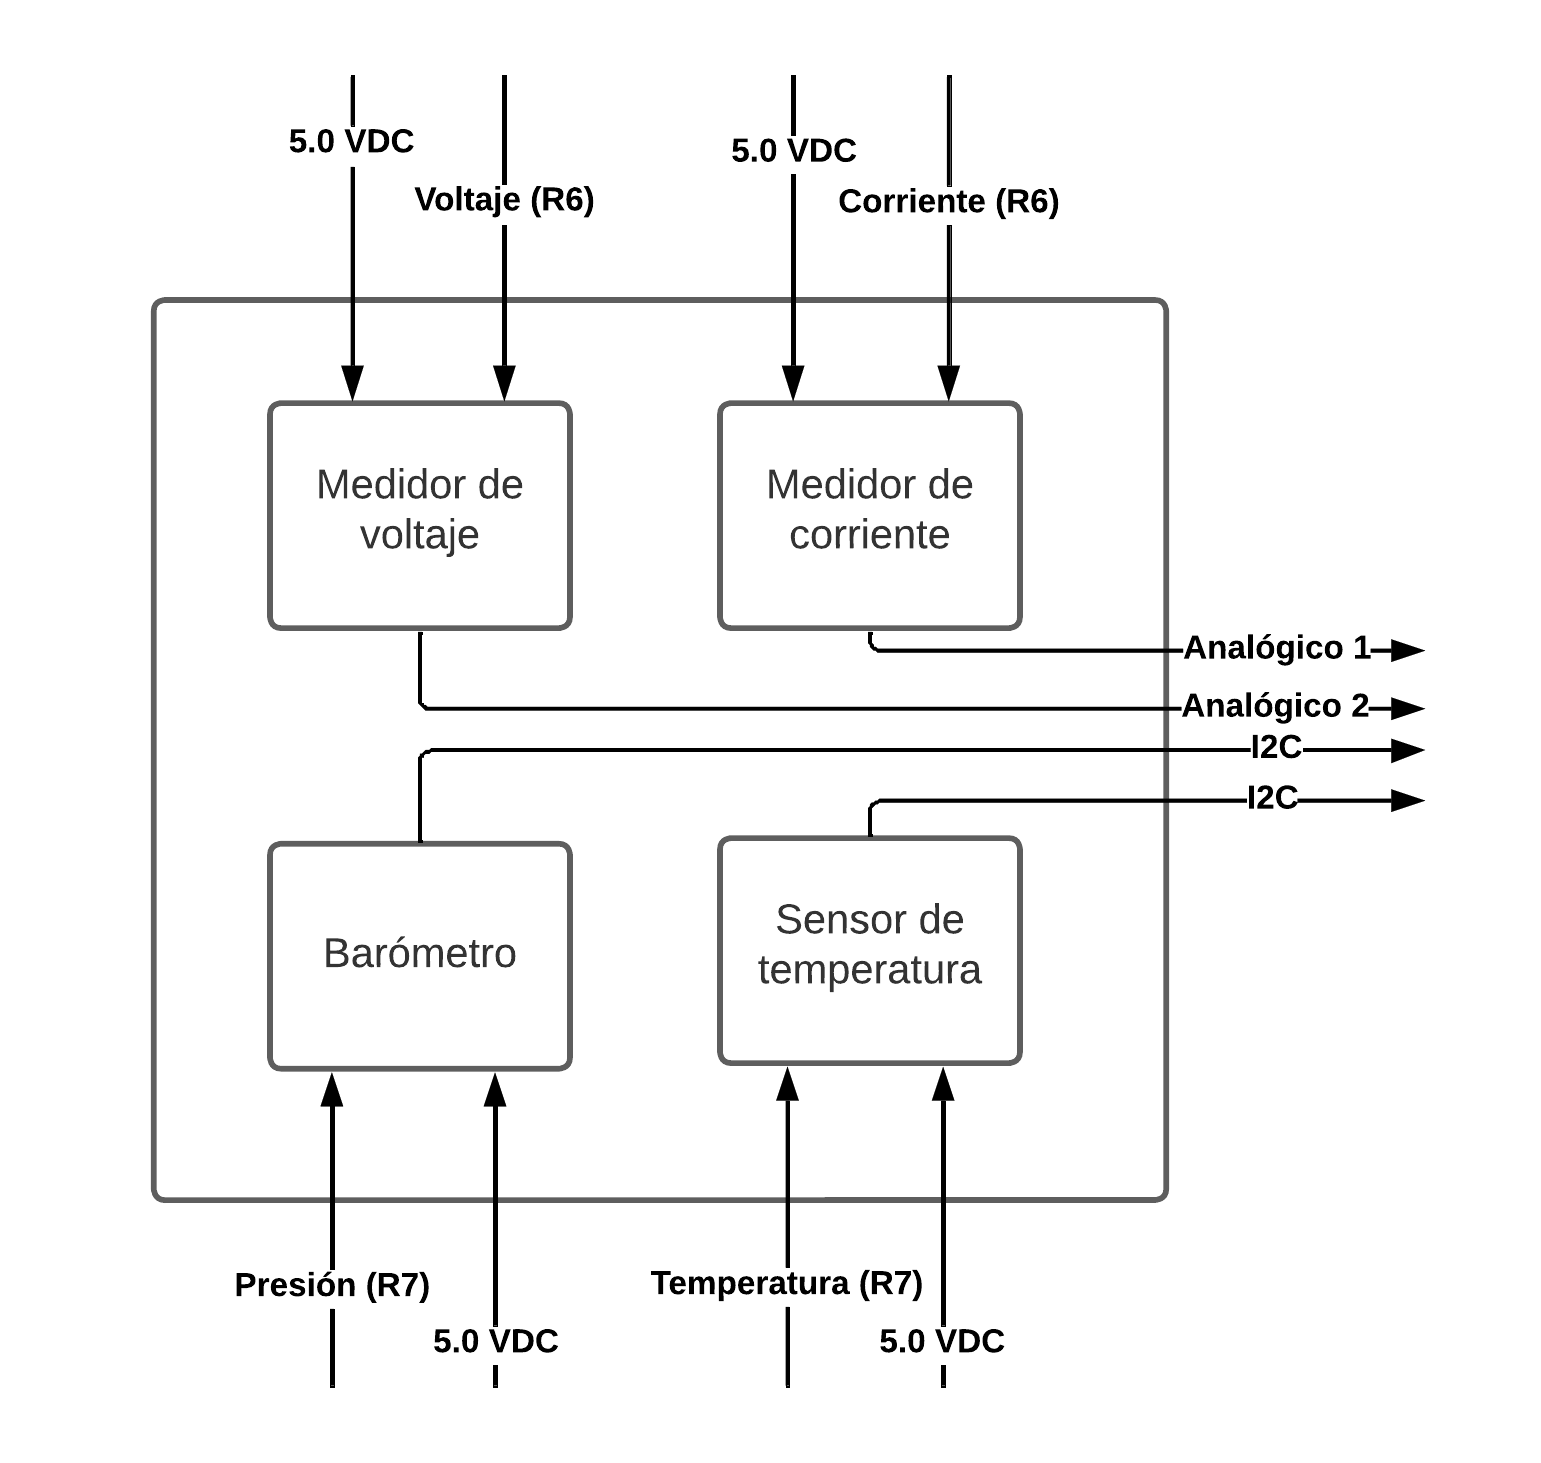
\includegraphics[width=\textwidth]{Pictures/Level2A.png}
\caption{Diagrama funcional Nivel 2, Instrumentación.}\label{fig:Level2A}
\index{figures}
\end{figure}

%**************************************
% BARÓMETRO

\begin{table}[h!]
    \centering
    \caption{Detalles de Nivel 1, Barómetro}
    \label{tab:nivel2_Barometro}
    \begin{tabular}{ll}
    \toprule
        Módulo  & Barómetro\\ 
    \midrule
        Entradas & 
        \begin{minipage}[t]{0.75\linewidth}
  - Alimentación $5.0 \, \text{V} \pm 1\%$\\
   - Presión atmosférica
 
        \end{minipage} \\
    \midrule
        Salidas & 
        \begin{minipage}[t]{0.75\linewidth}
    - Señal vía I2C

        \end{minipage} \\
    \midrule
        Funcionamiento & 
        \begin{minipage}[t]{0.75\linewidth}
El barómetro se alimenta con una tensión de $5.0 \, \text{V} \pm 1\%$. Transforma la presión atmosférica en una señal eléctrica, la acondiciona y posteriormente transmite los datos a través de la comunicación I2C.

        \end{minipage} \\
    \bottomrule
    \end{tabular}
\end{table}

%**************************************
% SENSOR DE TEMPERATURA 

\begin{table}[h!]
    \centering
    \caption{Detalles de Nivel 1, Sensor de temperatura}
    \label{tab:nivel2_Temperatura}
    \begin{tabular}{ll}
    \toprule
        Módulo  & Sensor de temperatura\\ 
    \midrule
        Entradas & 
        \begin{minipage}[t]{0.75\linewidth}
  - Alimentación $5.0 \, \text{V} \pm 1\%$\\
   - Temperatura ambiente
 
        \end{minipage} \\
    \midrule
        Salidas & 
        \begin{minipage}[t]{0.75\linewidth}
    - Señal vía I2C

        \end{minipage} \\
    \midrule
        Funcionamiento & 
        \begin{minipage}[t]{0.75\linewidth}
El sensor de temperatura se alimenta con una tensión de $5.0 \, \text{V} \pm 1\%$. Transforma la temperatura ambiente en una señal eléctrica, la acondiciona y posteriormente transmite los datos a través de la comunicación I2C.

        \end{minipage} \\
    \bottomrule
    \end{tabular}
\end{table}


%**************************************
% ADC

\begin{table}[h!]
    \centering
    \caption{Detalles de Nivel 1, Medidor de voltaje}
    \label{tab:nivel2_Voltaje}
    \begin{tabular}{ll}
    \toprule
        Módulo  & Medidor de voltaje\\ 
    \midrule
        Entradas & 
        \begin{minipage}[t]{0.75\linewidth}
  - Alimentación $5.0 \, \text{V} \pm 1\%$\\
   - Voltaje del banco de baterías
 
        \end{minipage} \\
    \midrule
        Salidas & 
        \begin{minipage}[t]{0.75\linewidth}
    - Señal analógica 2 - 10 bits.

        \end{minipage} \\
    \midrule
        Funcionamiento & 
        \begin{minipage}[t]{0.75\linewidth}
El ADC se alimenta con una tensión de $5.0 \, \text{V} \pm 1\%$. Este posee una resolución de 10 bits. 

        \end{minipage} \\
    \bottomrule
    \end{tabular}
\end{table}

%**************************************
% Sensor de corriente

\begin{table}[h!]
    \centering
    \caption{Detalles de Nivel 1, Medidor de corriente}
    \label{tab:nivel2_Voltaje}
    \begin{tabular}{ll}
    \toprule
        Módulo  & Medidor de corriente\\ 
    \midrule
        Entradas & 
        \begin{minipage}[t]{0.75\linewidth}
  - Alimentación $5.0 \, \text{V} \pm 1\%$\\
   - Corriente de banco de baterías.
 
        \end{minipage} \\
    \midrule
        Salidas & 
        \begin{minipage}[t]{0.75\linewidth}
    - Señal analógica 1.

        \end{minipage} \\
    \midrule
        Funcionamiento & 
        \begin{minipage}[t]{0.75\linewidth}
El medidor de corriente se alimenta con una tensión de $5.0 \, \text{V} \pm 1\%$. Utilizando el Efecto Hall, genera una señal de voltaje que se presenta como Analógica 1.


        \end{minipage} \\
    \bottomrule
    \end{tabular}
\end{table}